\documentclass[a4paper, 10pt]{report}
\usepackage[italian]{babel}
\usepackage{amsmath, amsfonts, amssymb, amsthm}
\usepackage{graphicx}
\usepackage{hyperref}
%\UseRawInputEncoding

\usepackage{listings}
\usepackage{color}
\definecolor{dkgreen}{rgb}{0,0.6,0}
\definecolor{gray}{rgb}{0.5,0.5,0.5}
\definecolor{mauve}{rgb}{0.58,0,0.82}
\lstset{frame=tb,
  language=Java,
  aboveskip=3mm,
  belowskip=3mm,
  showstringspaces=false,
  columns=flexible,
  basicstyle={\small\ttfamily},
  numbers=none,
  numberstyle=\tiny\color{gray},
  keywordstyle=\color{blue},
  commentstyle=\color{dkgreen},
  stringstyle=\color{mauve},
  breaklines=true,
  breakatwhitespace=true,
  tabsize=3
}

\begin{document}
\begin{figure}[t]

\includegraphics[scale=0.33,angle=0]{logo.png}
\newline
\centering{Facoltà di Ingegneria\\ Corso di Laurea in Ingegneria Informatica}
\end{figure}
\title{\Large{Elaborato Ingegneria del Software}\\ \Huge{\textbf{Applicazione in Java per la gestione della vendita di medicine in una farmacia}}}
\author{Athos Innocenti}
\date{A.A. 2019 - 2020}
\maketitle
\tableofcontents
\chapter{Introduzione}
L'obiettivo di questo progetto è realizzare un software in Java per la gestione della vendita di medicine in una farmacia.

Il cliente, interagendo con la farmacia, comunica il nome della medicina che vuole acquistare e se desidera la versione originale o generica. A questo punto viene controllata la disponibilità di tale medicina nel magazzino: se la medicina richiesta è disponibile si prosegue con il pagamento altrimenti viene creata una prenotazione a nome del cliente contenete i suoi dati e le informazioni relative alla medicina prenotata. Nella prima fase del pagamento viene chiesto al cliente se desidera pagare la medicina a prezzo pieno o con una riduzione: se desidera acquistare a prezzo pieno al costo della medicina viene aggiunta l'iva e un tasso di guadagno per la farmacia, se invece desidera acquistare a prezzo ridotto viene richiesto l'ISEE del cliente, si calcola la fascia di redditto di appartenenza e in base ad essa viene applicato uno sconto. Una volta acquistata o prenotata una medicina viene chiesto al cliente se desidera acquistarne un'altra. Conclusa l'interazione viene mostrato lo scontrino contenente un riassunto di tutte le medicine acquistate con il costo totale di esse e si passa al cliente successivo, se presente, altrimenti la farmacia chiude e viene fatto un resoconto sul guadagno totale.

Qualora la medicina richiesta non fosse disponibile, una funzione ne simula la richiesta alla casa farmaceutica e la conseguente acquisizione tramite la creazione di nuovi oggetti di tipo medicina a partire dalla lista di tutte le medicine richieste.

Per rappresentare una situazione più realistica possono essere create medicine richieste solo da clienti passati e non dal cliente attuale.

La medicina che il cliente vuole acquistare, la sua tipologia e la medicina richiesta che verrà creata sono tutte scelte casualmente.\\

Nella fase iniziale di progettazione sono stati individuati i vari casi d'uso che sono stati riportati all'interno dello use case diagram.

Insieme ai casi d'uso è stata definita una logica di dominio in prospettiva di implementazione che è stata rappresentata attraverso un diagramma UML.

Per la realizzazione del progetto sono stati utilizzati tre design patterns: il design pattern creazionale Singleton applicato alla classe Pharmacy rappresentante la farmacia; il design pattern comportamentale Observer tra la classe Pharmacy che riveste il ruolo di observer e la classe Warehouse, rappresentante il magazzino della farmacia, che riveste invece il ruolo di subject e il design pattern strutturale Proxy per il pagamento della medicina che il cliente desidera acquistare a seconda che quest'ultimo desideri pagare a prezzo pieno o ridotto.

Si è venuta quindi a creare una rappresentazione dell'interazione tra cliente e farmacia dove i vari attributi relativi al cliente, alla farmacia, ai farmacisti e la scelta del metodo di pagamento e la volontà di acquistare altre medicine sono inseriti da linea di comando mediante l'impiego di oggetti Scanner.

Il progetto durante tutta la sua progettazione e realizzazione è stato versionato con Git ed è disponibile su GitHub al seguente \href{https://github.com/athos-innocenti/Pharmacy}{\underline{\textbf{link}}}.
\chapter{Progettazione}
\section{Diagramma UML}
Si riporta il diagramma UML che descrive la logica di dominio in prospettiva di implementazione.
\begin{figure}[h]
\centering
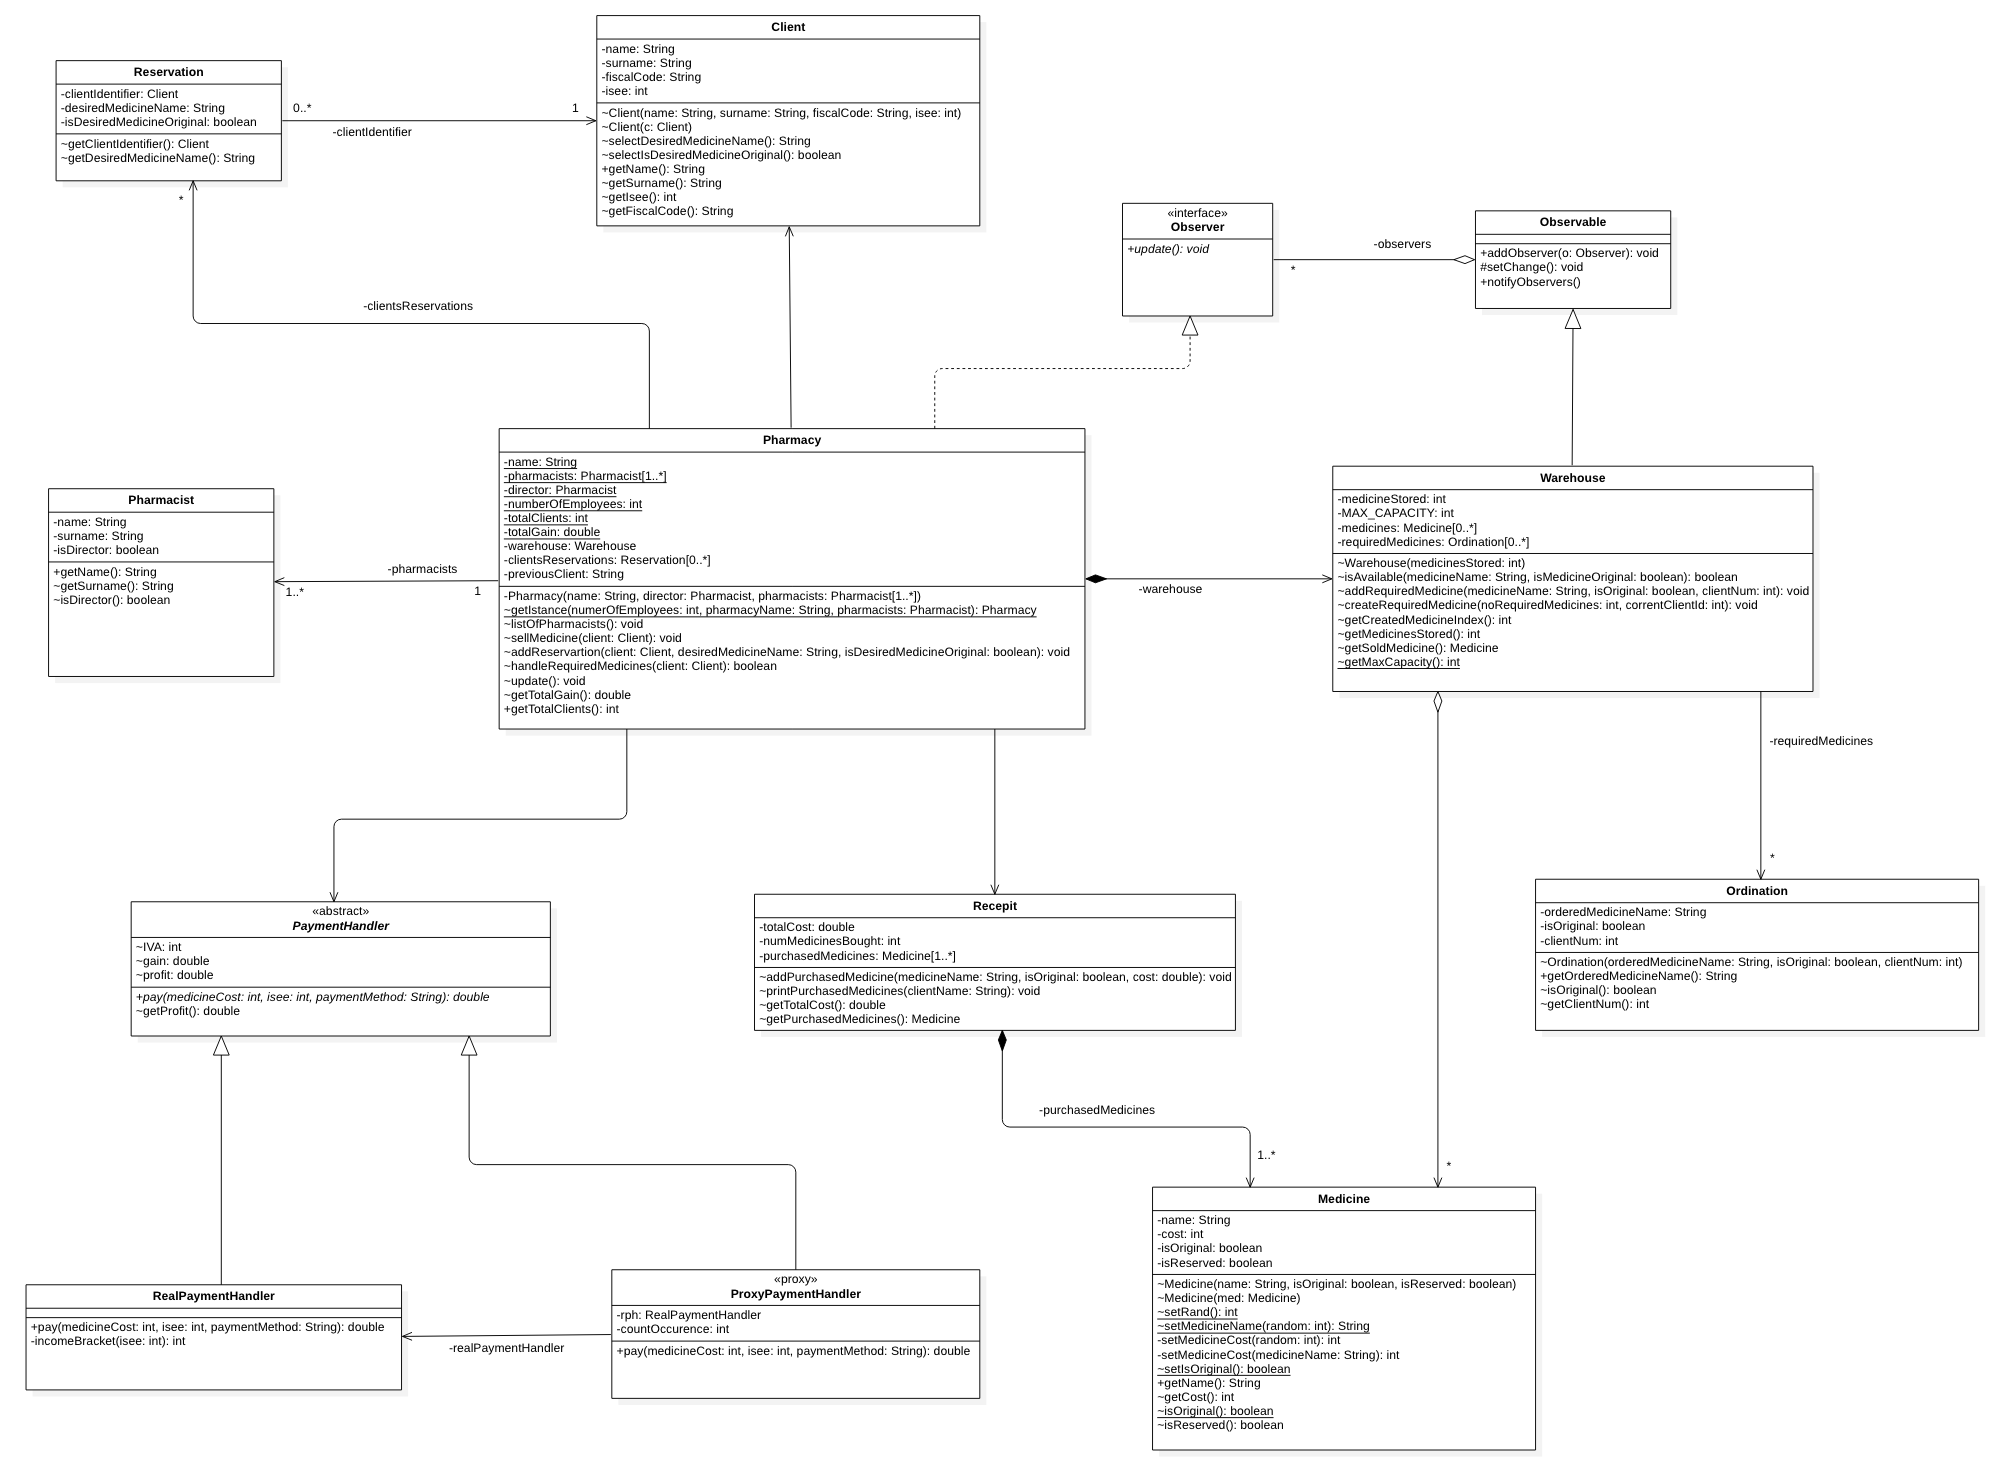
\includegraphics[scale=0.4,angle=0]{PharmacyUML.png}
\caption{Diagramma UML}
\end{figure}
\section{Use Case Diagram}
Si riporta uno Use Case Diagram composto da attore e vari casi d'uso.
\begin{figure}[h]
\centering
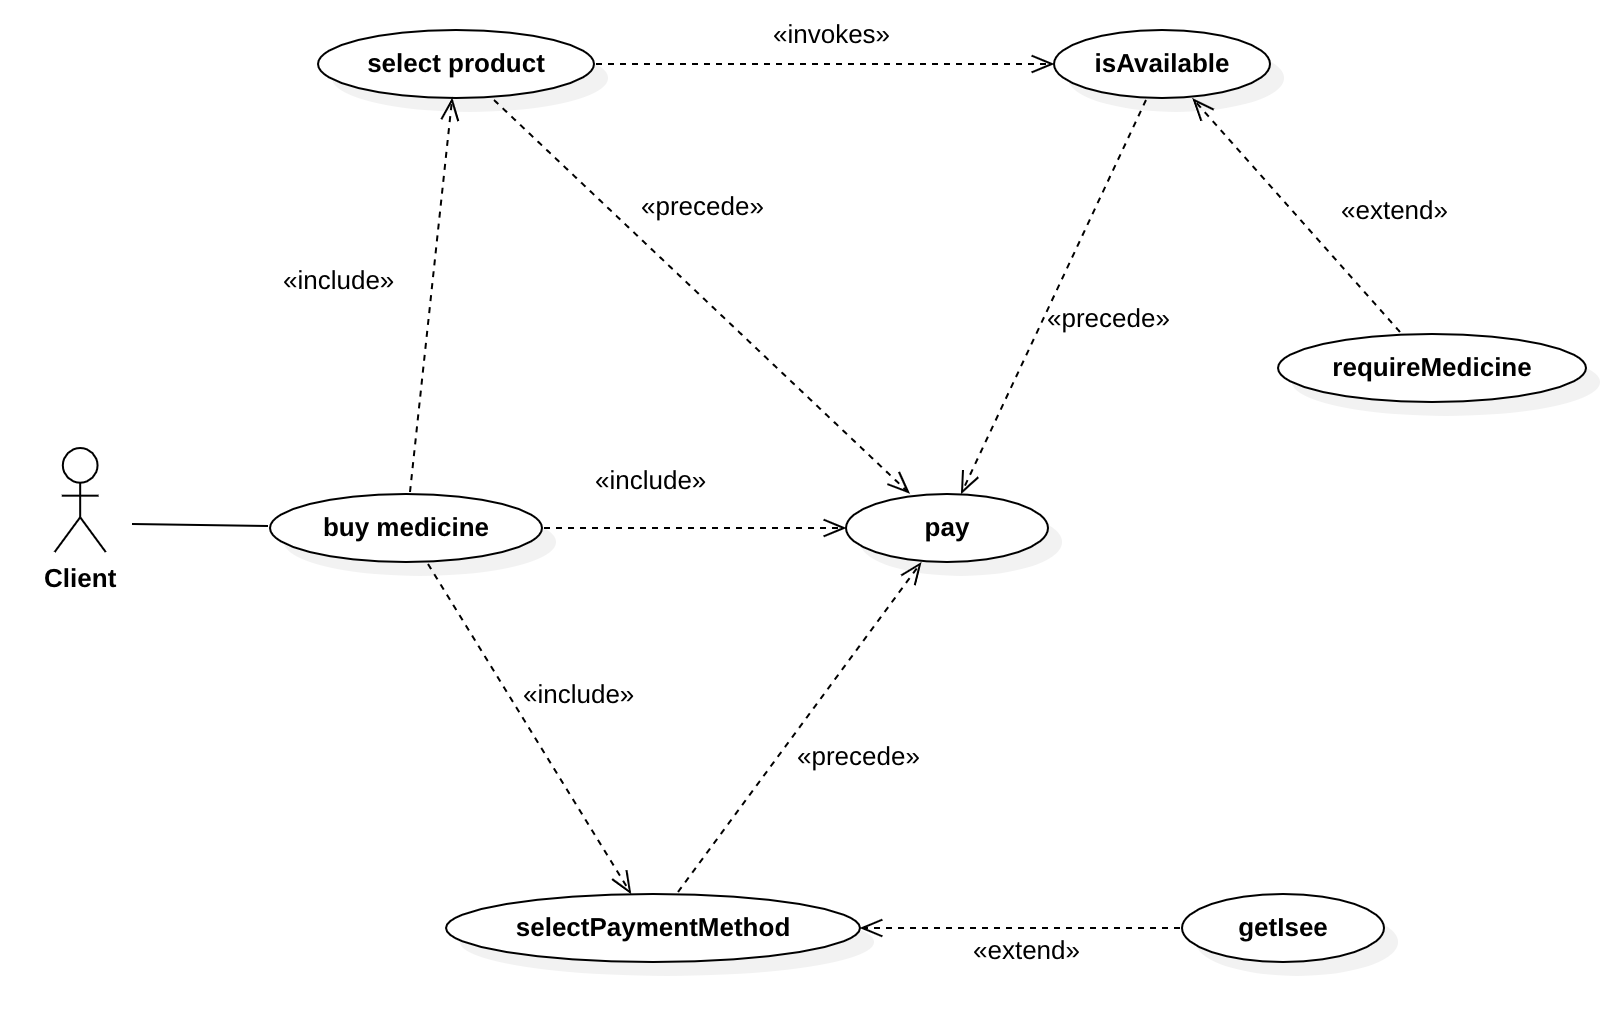
\includegraphics[scale=0.5,angle=0]{PharmacyUCD.png}
\caption{Use Case Diagram}
\end{figure}
\section{Sequence Diagram}
Si riporta qui di seguito (pagina successiva) un Sequence Diagram che simula l'esecuzione del programma considerando i diversi flussi di esecuzione possibili dipendenti dalla disponibilità o meno della medicina e dal metodo di pagamento scelto da parte del cliente.
\begin{figure}[t]
\centering
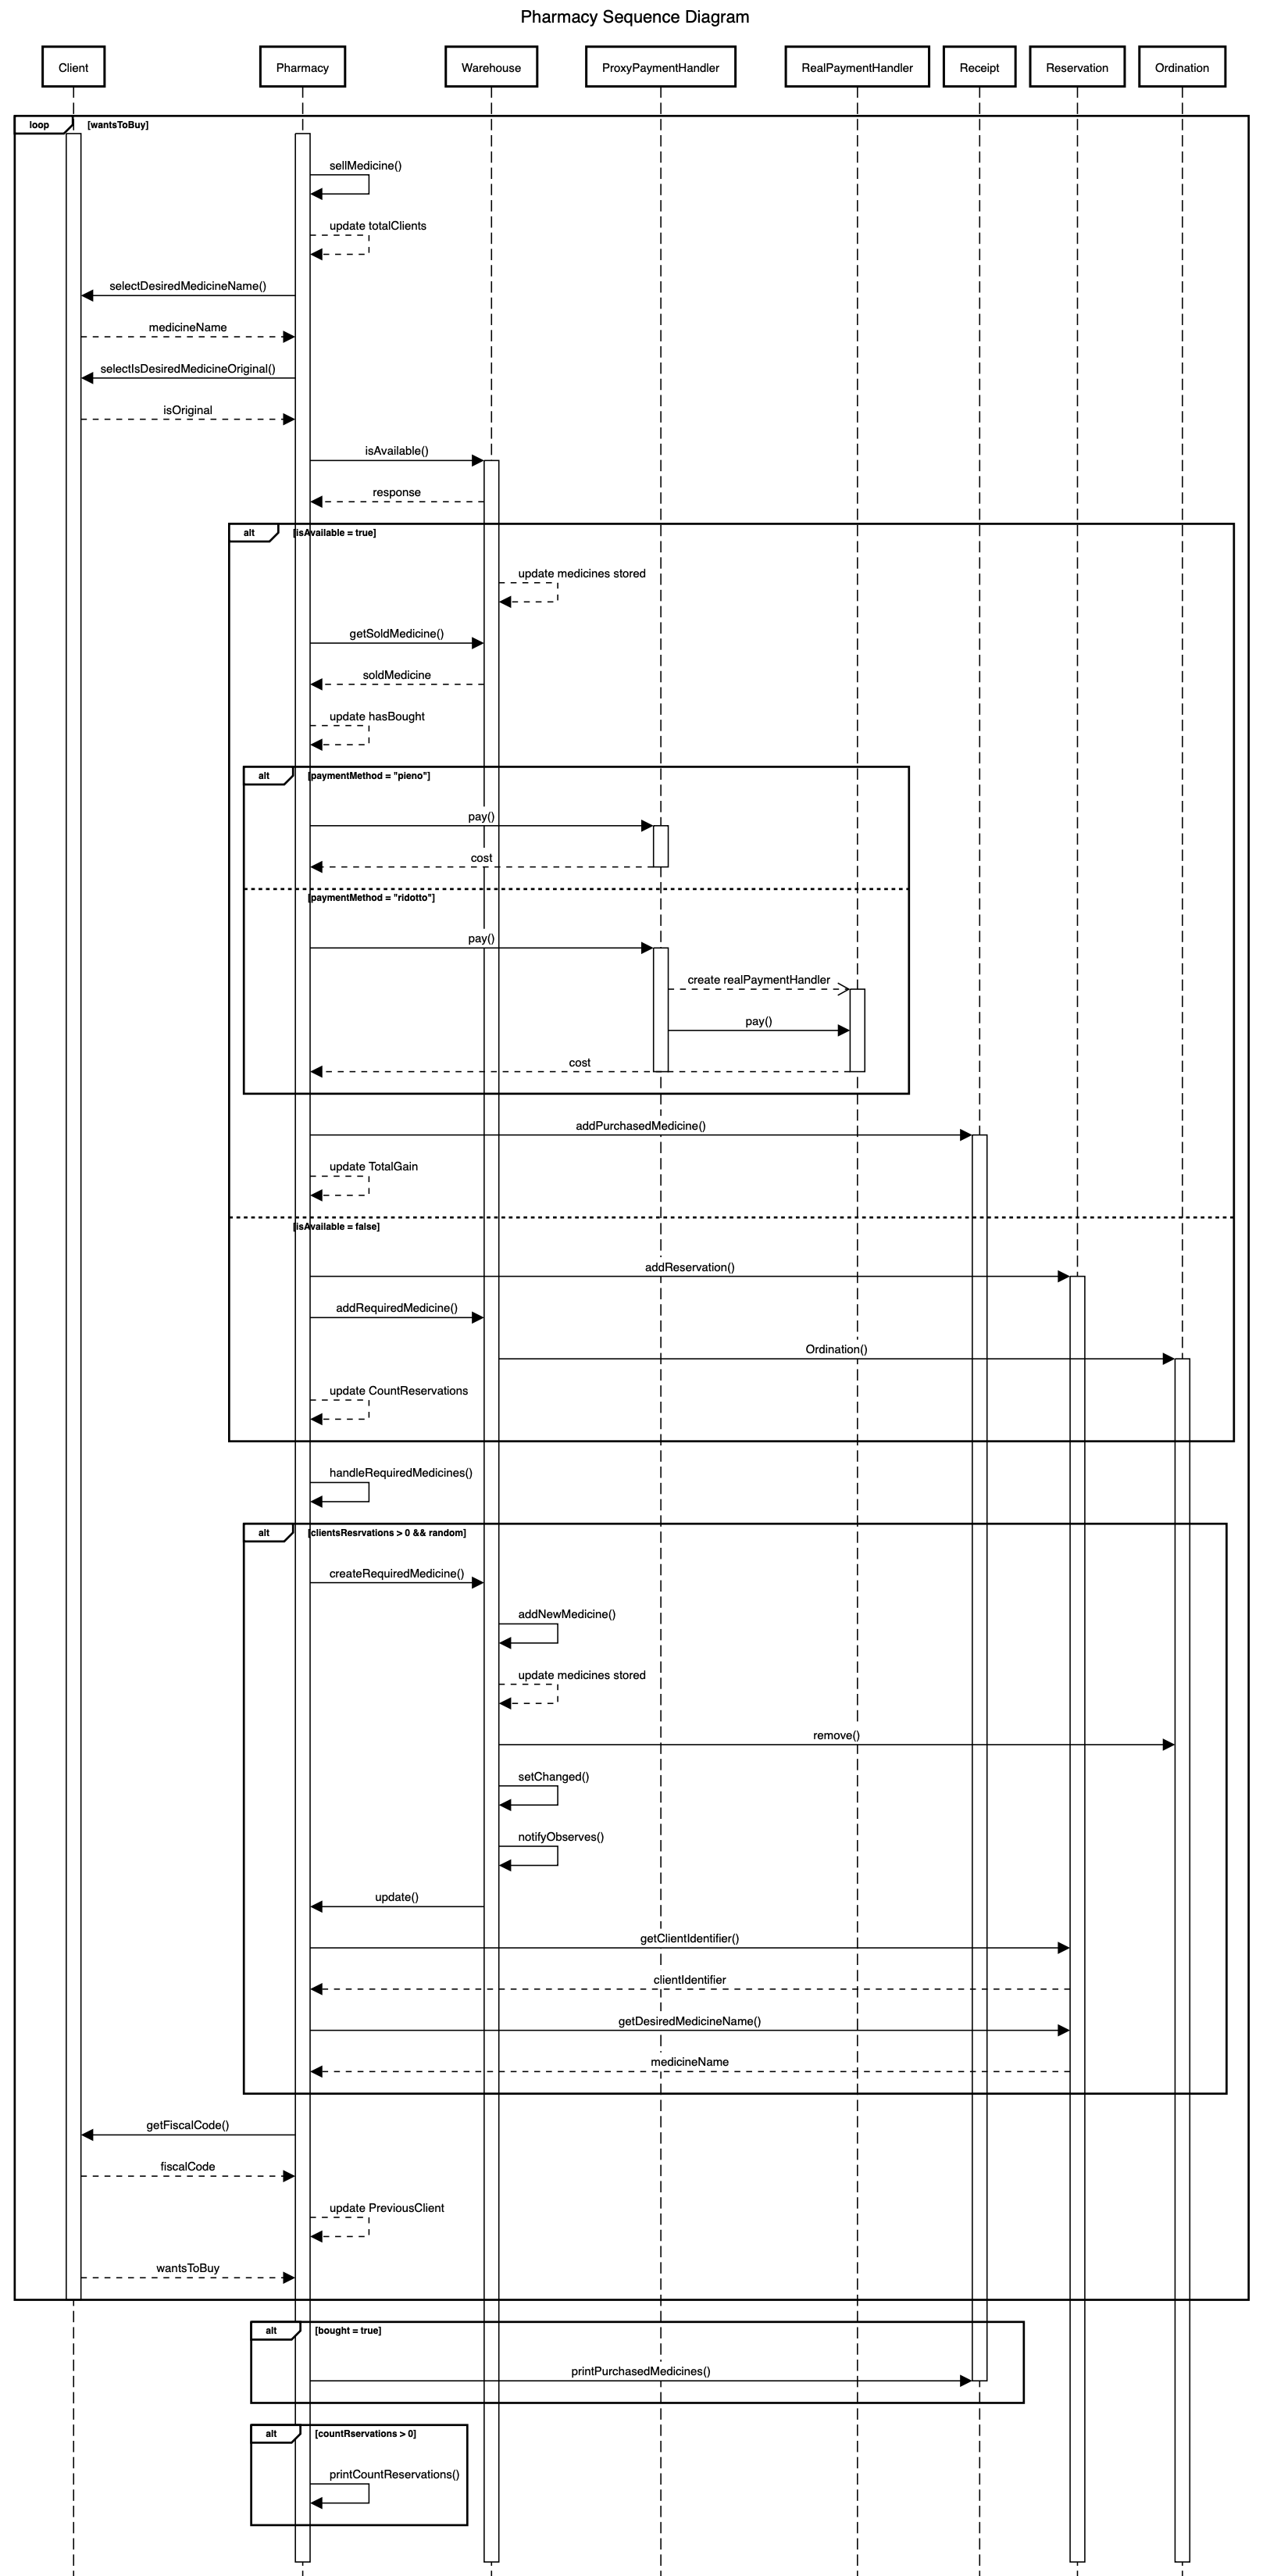
\includegraphics[scale=0.2,angle=0]{PharmacySD.png}
\caption{Sequence Diagram}
\end{figure}
\chapter{Realizzazione}
\section{Classi}
Vengono ora presentate tutte le classi facenti parte del progetto. Ne viene fornita una breve descrizione corredata di frammenti di codice (non vengono mostrati getter e setter).

Sono state definite 10 classi e una classe astratta per l'implementazione del design pattern Proxy. A queste si aggiungono la classe \textbf{Observable} e l'interfaccia \textbf{Observer} collocate nel package \textsc{java.util}.

Le classi del progetto sono:
\begin{enumerate}
\item Pharmacy
\item Pharmacist
\item Warehouse
\item Medicine
\item Client
\item ProxyPaymentHandler
\item RealPaymentHandler
\item Ordination
\item Reservation
\item Receipt
\end{enumerate}
\subsection{Pharmacy}
La classe \textbf{Pharmacy} è la classe principale dell'intero progetto e rappresenta la farmacia che si vuole gestire attraverso l'applicativo. È la classe \textit{Singleton} del progetto e funge da \textit{Observer} sul magazzino. Essendo un singleton ha un costruttore privato, gli attributi che la definiscono sono statici ed è dotata di un metodo statico \textsc{getIstance()} che restituisce la singola istanza della classe. Per poter creare l'oggetto si deve passare al costruttore il \textit{name} della farmacia, un array di farmacisti (\textit{pharmacists}) che rappresenta i farmacisti che lavorano presso quella farmacia, e il direttore (\textit{director}) della farmacia che corrisponde al primo farmacista nell'array.

Altri attributi che la caratterizzano sono:
\begin{enumerate}
\item \textit{totalClients}: intero che conta il numero totale di clienti
\item \textit{totalGain}: il guadagno totale della farmacia. Viene aggiornato ogni volta che un cliente acquista una nuova medicina
\item \textit{clientsReservations}: ArrayList di prenotazioni create quando un cliente desidera acquistare una medicina non disponibile. Contiene informazioni utili per poter notificare il cliente quando la medicina richiesta sarà disponibile.
\item \textit{warehouse}: il magazzino della farmacia
\end{enumerate}
La funzione \textsc{sellMedicine()} è la funzione cardine del progetto e si occupa della interazione con il cliente nonché della vendita delle medicine. Viene inizialmente richiesto al cliente il nome e la tipologia di medicina che vuole acquistare. A questo punto viene invocato il metodo \textsc{isAvailable()} del magazzino che verifica la disponibilità della medicina richiesta e, in caso positivo, la rende fruibile. Se la medicina non è disponibile viene invocato il metodo \textsc{addReservation()}, altrimenti si procede con il pagamento chiedendo al cliente se desidera pagare a prezzo pieno o ridotto. A seguito della risposta del cliente, se è la prima medicina acquistata dal cliente viene creato un nuovo scontrino (\textit{receipt}) che terrà traccia di tutte le medicine acquistate dal cliente e un nuovo \textit{ProxyPaymentHandler}, se invece il cliente ha già acquistato altre medicine vengono usati i due oggetti già creati. Concluse tutte queste operazioni si chiede al cliente se vuole acquistare un'altra medicina: in caso affermativo si ripete l'intera procedura, altrimenti il metodo si conclude.

La funzione \textsc{addReservation()} aggiunge una nuova prenotazione a nome del cliente corrente per la medicina attualmente non disponibile che vuole acquistare. Inoltre crea anche una nuova ordinazione per il magazzino.

La funzione \textsc{handleRequiredMedicines()} stabilisce se creare o meno una nuova medicina richiesta. Se il cliente attuale è almeno il secondo e se c'è almeno una prenotazione si va a controllare che ne esista almeno una per un cliente precedente a quello attuale e, in caso positivo, viene invocato il metodo \textsc{createRequiredMedicine()} del magazzino. Viene fatto questo controllo per impedire che vengano create medicine richieste dal cliente attuale poiché questo scenario sarebbe del tutto irrealistico.

Infine, la funzione \textsc{update()} è l'implementazione della omonima funzione dell'interfaccia \textit{Observer}. Notifica il cliente interessato che una medicina da lui richiesta è ora disponibile nel magazzino e si occupa di eliminare la corrispondente prenotazione in \textit{clientsReservations}. Viene implementato l'observer tipo pull in cui il \textit{Subject} notifica l’\textit{Observer} che lo stato è cambiato ma poi è l’\textit{Observer} a chiamare un metodo per leggere lo stato. In questo caso viene usato il metodo \textsc{getCreatedMedicineIndex()} per sapere quale medicina è stata creata.\\
\begin{lstlisting}
public class Pharmacy implements Observer {
    private static String name;
    private static Pharmacist[] pharmacists;
    private static Pharmacist director;
    private static double totalGain;
    private static int totalClients;
    private static int numberOfEmployees;

    private static Warehouse warehouse;
    private static ArrayList<Reservation> clientsReservations;

    private static Scanner scanner = new Scanner(System.in);
    private static Pharmacy istance = null;

    private static String previousClient;
    private PaymentHandler payment;
    private Receipt receipt;

    private Pharmacy(String name, Pharmacist director, Pharmacist[] pharmacists) {
        Pharmacy.name = name;
        Pharmacy.director = director;
        Pharmacy.pharmacists = pharmacists;

        totalGain = 0;
        totalClients = 0;
        clientsReservations = new ArrayList<>();
        previousClient = "";

        warehouse = new Warehouse((int) (Math.random() * (Warehouse.getMaxCapacity() + 1) + 1));
        warehouse.addObserver(this);
    }

    static Pharmacy getIstance(int numberOfEmployees, String pharmacyName, Pharmacist[] pharmacists) {
        if (istance == null) {
            istance = new Pharmacy(pharmacyName, pharmacists[0], pharmacists);
            Pharmacy.setNumberOfEmployees(numberOfEmployees);
        }
        return istance;
    }

    void sellMedicine(Client client) throws FullWarehouseException {
        totalClients++;
        String desiredMedicineName;
        int countReservations = 0;
        int previousReservations = 0;
        boolean bought = false;
        boolean isDesiredMedicineOriginal, wantsToBuy, hasBought;
        do {
            desiredMedicineName = client.selectDesiredMedicineName();
            isDesiredMedicineOriginal = client.selectIsDesiredMedicineOriginal();
            hasBought = bought;
            if (warehouse.isAvailable(desiredMedicineName, isDesiredMedicineOriginal)) {
                bought = true;
                System.out.println("Medicina richiesta disponibile nel magazzino");
                System.out.println("Si desidera acquistare a prezzo pieno o ridotto? (pieno o ridotto)");
                String paymentMethod = scanner.nextLine();
                if (!client.getFiscalCode().equals(previousClient) || (previousReservations < countReservations && !hasBought)) {
                    payment = new ProxyPaymentHandler();
                    receipt = new Receipt();
                }
                double cost = payment.pay(warehouse.getSoldMedicine().getCost(), client.getIsee(), paymentMethod);
                receipt.addPurchasedMedicine(desiredMedicineName, isDesiredMedicineOriginal, cost);
                totalGain += cost;
                System.out.println("\nVenduta la medicina: " + warehouse.getSoldMedicine().getName() + " al prezzo di: " + cost);
                System.out.println(client.getName() + " ha speso finora: " + payment.getProfit() + "\n");
                System.out.println("Il magazzino contiene ora " + warehouse.getMedicinesStored() + " medicine");
            } else {
                previousReservations = countReservations;
                countReservations++;
                addReservation(client, desiredMedicineName, isDesiredMedicineOriginal);
            }
            handleRequiredMedicines(client);
            System.out.println("\nSi vuole acquistare un'altra medicina? (si o no)");
            wantsToBuy = scanner.nextLine().equals("si");
            previousClient = client.getFiscalCode();
        }
        while (wantsToBuy);
        if (bought) {
            receipt.printPurchasedMedicines(client.getName());
            System.out.println("Spende in totale: " + receipt.getTotalCost());
        }
        if (countReservations > 0) {
            System.out.println(client.getName() + " ha " + countReservations + " medicine prenotate");
        }
    }

    void addReservation(Client client, String desiredMedicineName, boolean isDesiredMedicineOriginal) {
        System.out.println("Medicina richiesta non disponibile");
        clientsReservations.add(new Reservation(new Client(client), desiredMedicineName, isDesiredMedicineOriginal));
        System.out.println("Creata una prenotazione a nome: " + client.getName() + " per la medicina: " + desiredMedicineName + "\n");
        warehouse.addRequiredMedicine(desiredMedicineName, isDesiredMedicineOriginal, totalClients);
    }

    boolean handleRequiredMedicines(Client client) throws FullWarehouseException {
        boolean random = Math.random() < 0.5;
        if (totalClients > 1 && clientsReservations.size() > 0 && random) {
            for (Reservation r : clientsReservations) {
                if (!r.getClientIdentifier().getFiscalCode().equals(client.getFiscalCode())) {
                    warehouse.createRequiredMedicine(clientsReservations.size() - 1, totalClients - 1);
                    break;
                }
            }
        }
        return random;
    }

    @Override
    public void update(Observable o, Object arg) {
        int index = warehouse.getCreatedMedicineIndex();
        String clientName = clientsReservations.get(index).getClientIdentifier().getName();
        String medicineName = clientsReservations.get(index).getDesiredMedicineName();
        System.out.println("AVVISATO IL CLIENTE " + clientName + " CHE VIENE RISERVATA LA MEDICINA " + medicineName + "!\n");
        clientsReservations.remove(index);
    }

    double getTotalGain() {
        BigDecimal bd = new BigDecimal(Double.toString(totalGain));
        bd = bd.setScale(2, BigDecimal.ROUND_FLOOR);
        return bd.doubleValue();
    }
}
\end{lstlisting}
\subsection{Pharmacist}
La classe \textbf{Pharmacist} rappresenta un farmacista che lavora nella farmacia in esame. Oltre agli attributi \textit{name} e \textit{surname}, a ciascun farmacista è associato l'attributo booleano \textit{isDirector} che indica se il farmacista è o meno il direttore della farmacia.

La definizione del numero di farmacisti che lavorano nella farmacia e la conseguente creazione di ognuno di essi, e quindi anche la creazione del direttore, precedono e sono necessarie per la creazione della farmacia.\\
\begin{lstlisting}
public class Pharmacist {
    private final String name;
    private final String surname;
    private final boolean isDirector;

    Pharmacist(String name, String surname, boolean isDirector) {
        this.name = name;
        this.surname = surname;
        this.isDirector = isDirector;
    }
}
\end{lstlisting}
\subsection{Warehouse}
La classe \textbf{warehouse} rappresenta il magazzino della farmacia. 

Gli attributi della classe sono:
\begin{enumerate}
\item \textit{medicinesStored}: intero che conta il numero di medicine che si trovano all'interno del magazzino
\item \textit{max capacity}: costante che indica il numero massimo di medicine che il magazzino può contenere. Se la capacità massima viene superata viene lanciata l'eccezione \textbf{FullWarehouseException}
\item \textit{medicines}: ArrayList di medicine che tiene traccia di tutte le medicine contenute nel magazzino. Viene creato e popolato quando viene inizializzato il magazzino e le nuove medicine ottenute su richiesta del cliente sono collocate al suo interno e contrassegnate come riservate
\item \textit{soldMedicine}: tiene traccia della medicina che è stata appena venduta
\item \textit{requiredMedicines}: ArrayList di ordinazioni contenente tutte le medicine ordinate, ovvero tutte le medicine che i vari clienti volevano acquistare ma che non erano disponibili nel magazzino. Quando la medicina diventa disponibile, l'ordinazione associata viene eliminata.
\end{enumerate}
Le medicine che si trovano inizialmente all'interno del magazzino sono create in modo casuale tramite il costruttore di default \textsc{Medicine()}. Anche il numero di medicine inizialmente disponibili è casuale e stabilito entro l'intervallo 0 - \textit{max capacity}. 

La funzione \textsc{isAvailable()} riceve in ingresso il nome e la tipologia della medicina che il cliente corrente vuole acquistare. Tramite un ciclo for si scansiona l'ArrayList \textit{medicines} per verificare se la medicina richiesta è disponibile, in tal caso la medicina viene rimossa dall'ArrayList, il contatore \textit{medicinesStored} viene decrementato e la medicina venduta viene memorizzata in \textit{soldMedicine} tramite costruttore di copia.

La funzione \textsc{addRequiredMedicine()} crea una nuova ordinazione inserita nell'ArrayList \textit{requiredMedicines} con i dati relativi alla medicina da richiedere e il numero del cliente.

Infine, la funzione \textsc{createRequiredMedicine()} crea una delle medicine che sono state richieste dai clienti. Possono essere create solo le medicine richieste da clienti precedenti a quello attuale e la medicina creata è scelta in modo casuale. Nel momento in cui la medicina richiesta viene creata questa viene aggiunta al magazzino (quindi in \textit{medicines}), viene incrementato il numero di medicine nel magazzino e l'ordinazione ad essa associata viene eliminata. È a questo punto che entra in gioco il design pattern observer in quanto verranno invocate le funzioni \textsc{setChanged()} e \textsc{notifyObservers()} per notificare l'\textit{Observer}, la classe \textbf{Pharmacy}, che una medicina richiesta è ora disponibile.\\
\begin{lstlisting}
class Warehouse extends Observable {
    private int medicinesStored, createdMedicineIndex;
    private static final int MAX_CAPACITY = 100;
    private ArrayList<Medicine> medicines = new ArrayList<>();
    private Medicine soldMedicine;
    private ArrayList<Ordination> requiredMedicines = new ArrayList<>();

    Warehouse(int medicinesStored) {
        this.medicinesStored = medicinesStored;
        for (int i = 0; i < medicinesStored; i++) {
            medicines.add(new Medicine());
        }
        System.out.println("\nIl magazzino contiene inizialmente " + medicinesStored + " medicine");
    }

    boolean isAvailable(String medicineName, boolean isMedicineOriginal) {
        boolean isAvailable = false;
        for (int i = 0; i < medicines.size(); i++) {
            if (medicineName.equals(medicines.get(i).getName()) && isMedicineOriginal == medicines.get(i).isOriginal() && !medicines.get(i).isReserved()) {
                isAvailable = true;
                soldMedicine = new Medicine(medicines.get(i));
                medicines.remove(i);
                medicinesStored--;
                break;
            }
        }
        return isAvailable;
    }

    void addRequiredMedicine(String medicineName, boolean isOriginal, int clientNum) {
        System.out.println("Medicina: " + medicineName + " richiesta alla casa farmaceutica");
        requiredMedicines.add(new Ordination(medicineName, isOriginal, clientNum));
    }

    void createRequiredMedicine(int noRequiredMedicines, int currentClientId) throws FullWarehouseException {
        if (medicinesStored < MAX_CAPACITY) {
            int randMed = (int) (Math.random() * noRequiredMedicines);
            if (requiredMedicines.get(randMed).getClientNum() != currentClientId) {
                medicines.add(new Medicine(requiredMedicines.get(randMed).getOrderedMedicineName(), requiredMedicines.get(randMed).isOrginal(), true));
                System.out.println("\nUNA MEDICINA PRENOTATA ORA DISPONIBILE!");
                createdMedicineIndex = randMed;
                requiredMedicines.remove(randMed);
                medicinesStored++;
            }
        } else {
            throw new FullWarehouseException();
        }
        setChanged();
        notifyObservers();
    }
}
\end{lstlisting}
\subsection{Medicine}
La classe \textbf{Medicine} rappresenta la generica medicina.

Gli attributi caratterizzanti la classe sono:
\begin{itemize}
\item \textit{name}: il nome della medicina
\item \textit{cost}: intero che indica il costo della medicina
\item \textit{isOriginal}: booleano che indica se la medicina è originale o generica
\item \textit{isReserved}: booleano che indica se la medicina è riservata. Questo attributo sarà sempre \textsc{false} ed eccezione del caso in cui la medicina è una medicina che un cliente voleva acquistare ma che non era momentaneamente disponibile ed è quindi stata richiesta alla casa farmaceutica
\end{itemize}
La classe ha tre possibili costruttori:
\begin{enumerate}
\item Il costruttore di default: è invocato nel momento in cui viene istanziato il magazzino per creare le medicine (il cui numero è scelto casualmente entro un intervallo preimpostato) contenute al suo interno e che quindi possono essere acquistate dai clienti. Con questo costruttore l'attributo \textit{isReserved} viene sempre settato a \textsc{false} mentre l'attributo \textit{isOriginal} viene settato casualmente. Per \textit{name} e \textit{cost} viene prima chiamata la funzione \textsc{setRand()} che conta tutte le possibili medicine che possono essere create e sceglie, casualmente, l'indice corrispondente ad una di esse. A partire da tale indice, rappresentato dall'intero \textit{rand}, si vanno a leggere il nome e il rispettivo prezzo della medicina associata all'indice rand
\item Il costruttore con parametri \textit{name}, \textit{isOriginal} e \textit{isReserved}: usato dalla classe Warehouse per creare le medicine richieste ma non disponibili e per aggiungere le medicine acquistate nello scontrino. Nel primo caso l'attributo \textsc{isReserved} verrà settato a \textsc{true}
\item Il costruttore di copia
\end{enumerate}
I metodi della classe sono: \textsc{setMedicineName()} e \textsc{setMedicineCost()} che, in funzione dell'intero \textit{rand}, settano nome e costo della medicina, e \textsc{setRand()} già discusso. In particolare, del metodo \textsc{setMedicineCost()} ne è stato fatto l'overload.\\
\begin{lstlisting}
public class Medicine {
    private final String name;
    private final int cost;
    private final boolean isOriginal;
    private final boolean isReserved;

    Medicine() {
        int rand = setRand();
        this.name = setMedicineName(rand);
        this.cost = setMedicineCost(rand + 1);
        this.isOriginal = setIsOriginal();
        this.isReserved = false;
    }

    Medicine(String name, boolean isOriginal, boolean isReserved) {
        this.name = name;
        this.cost = setMedicineCost(name);
        this.isOriginal = isOriginal;
        this.isReserved = isReserved;
    }

    Medicine(Medicine med) {
        this.name = med.getName();
        this.cost = med.getCost();
        this.isOriginal = med.isOriginal();
        this.isReserved = med.isReserved();
    }

    static int setRand() {
        int rand = 0;
        try {
            Scanner scanner = new Scanner(new File("src/data/medicinesList.txt"));
            int countLines = 0;
            while (scanner.hasNextLine()) {
                countLines++;
                scanner.nextLine();
            }
            scanner.close();
            rand = (int) (Math.random() * countLines + 1);
            if (rand % 2 == 0) {
                rand -= 1;
            }
        } catch (FileNotFoundException e) {
            System.out.println("File not found!");
        }
        return rand;
    }

    static String setMedicineName(int random) {
        String name = "";
        int indexLine = 1;
        try {
            Scanner scannerName = new Scanner(new File("src/data/medicinesList.txt"));
            while (indexLine != random) {
                scannerName.nextLine();
                indexLine += 1;
            }
            name = scannerName.nextLine();
            scannerName.close();
        } catch (FileNotFoundException e) {
            System.out.println("File not found!");
        }
        return name;
    }

    private int setMedicineCost(int random) {
        int indexLine = 1;
        int cost = 0;
        try {
            Scanner scannerCost = new Scanner(new File("src/data/medicinesList.txt"));
            while (indexLine != random) {
                scannerCost.nextLine();
                indexLine += 1;
            }
            cost = Integer.parseInt(scannerCost.nextLine());
            scannerCost.close();
        } catch (FileNotFoundException e) {
            System.out.println("File not found!");
        }
        return cost;
    }

    private int setMedicineCost(String medicineName) {
        int cost = 0;
        try {
            Scanner scanner = new Scanner(new File("src/data/medicinesList.txt"));
            while (scanner.hasNextLine()) {
                if (scanner.nextLine().equals(medicineName)) {
                    cost = Integer.parseInt(scanner.nextLine());
                    break;
                }
                scanner.nextLine();
            }
            scanner.close();
        } catch (FileNotFoundException e) {
            System.out.println("File not found!");
        }
        return cost;
    }

    static boolean setIsOriginal() {
        return (Math.random() < 0.5);
    }
}
\end{lstlisting}
\subsection{Client}
La classe \textbf{Client} rappresenta il cliente della farmacia che desidera acquistare una o più medicine.

I suoi attributi sono: \textit{name}, \textit{surname}, \textit{fiscalCode} (necessario per identificare il cliente durante i vari pagamenti e per la creazione di eventuali prenotazioni) e l'intero \textit{isee} necessario per stabilire la fascia di reddito per eventuali agevolazioni al momento del pagamento.

Tramite i metodi \textsc{selectDesiredMedicineName()} e \textsc{selectIsDesiredMedicineOriginal()} si stabiliscono, casualmente, il nome della medicina che il cliente vuole acquistare e la tipologia della medicina (originale o generica), dunque le varie medicine che il cliente vuole acquistare sono scelte casualmente in un campionario di medicine possibili. La classe è dotata anche del costruttore di copia usato per la creazione di una prenotazione.\\
\begin{lstlisting}
public class Client {
    private final String name;
    private final String surname;
    private final String fiscalCode;
    private final int isee;

    Client(String name, String surname, String fiscalCode, int isee) {
        this.name = name;
        this.surname = surname;
        this.fiscalCode = fiscalCode;
        this.isee = isee;
    }

    Client(Client c) {
        this.name = c.getName();
        this.surname = c.getSurname();
        this.fiscalCode = c.getFiscalCode();
        this.isee = c.getIsee();
    }

    String selectDesiredMedicineName() {
        String nameDesriedMedicine = Medicine.setMedicineName(Medicine.setRand());
        System.out.println("\n" + getName() + " vuole acquistare la medicina: " + nameDesriedMedicine);
        return nameDesriedMedicine;
    }

    boolean selectIsDesiredMedicineOriginal() {
        return Medicine.setIsOriginal();
    }
}
\end{lstlisting}
\subsection{ProxyPaymentHandler}
La classe \textbf{ProxyPaymentHandler} costituisce la classe \textit{Proxy} nell'omonimo design pattern. Ha un riferimento privato ad un oggetto \textit{RealPaymentHandler} che viene istanziato solo nel caso in cui il cliente decide di eseguire un pagamento ridotto. Se, durante l'interazione con il medesimo cliente, l'oggetto \textit{RealPaymentHandler}  è già stato creato, la classe non ne crea uno nuovo ma utilizza quello creato in precedenza. Tale controllo è fatto utilizzando l'attributo \textit{countOccurence} introdotto anche per ragioni legate ai tests condotti su questa classe.

Viene creato un solo oggetto di questa classe per cliente e viene creato nel momento in cui il cliente paga per la prima volta una medicina richiesta e disponibile in magazzino. Se tutte le medicine che il cliente desidera acquistare non sono disponibili, questo oggetto, e conseguentemente il \textit{RealPaymentHandler}, non viene mai creato per quel cliente.\\
\begin{lstlisting}
public class ProxyPaymentHandler extends PaymentHandler {
    private RealPaymentHandler realPaymentHandler;
    private int countOccurence;

    ProxyPaymentHandler() {
        super();
        this.countOccurence = 0;
        System.out.println("\nAvvio pagamento...");
    }

    public double pay(int medicineCost, int isee, String paymentMethod) {
        double cost;
        if (paymentMethod.equals("pieno")) {
            System.out.println("Pagamento " + paymentMethod + " avviato");
            cost = medicineCost + ((IVA / (double) 100) * medicineCost) + (gain * medicineCost);
            profit += cost;
        } else {
            if (countOccurence == 0) {
                realPaymentHandler = new RealPaymentHandler();
                countOccurence++;
            }
            cost = realPaymentHandler.pay(medicineCost, isee, paymentMethod);
            profit += cost;
        }
        return cost;
    }
\end{lstlisting}
\subsection{RealPaymentHandler}
La classe \textbf{RealPaymentHandler} costituisce la classe \textit{RealSubject} del design pattern Proxy. Rappresenta quindi la classe oggetto del forwarding da parte del \textit{ProxyPaymentHandler} e del lazy load. Implementa la funzione \textsc{pay()} della classe astratta \textit{PaymentHandler} per il pagamento della medicina con agevolazione. Tramite la funzione \textsc{incomeBracket()}, che riceve in ingresso l'isee del cliente, si stabilisce a quale delle quattro fasce di reddito appartiene il cliente; questa informazione viene poi usata all'interno della funzione \textsc{pay()} per applicare una riduzione sul prezzo della medicina.\\
\begin{lstlisting}
public class RealPaymentHandler extends PaymentHandler {

    RealPaymentHandler() {
        super();
    }

    public double pay(int medicineCost, int isee, String paymentMethod) {
        System.out.println("Pagamento " + paymentMethod + " avviato");
        int noBracket = incomeBracket(isee);
        double cost = medicineCost + ((IVA / (double) 100) * medicineCost) + (gain * medicineCost) - ((((4 - noBracket) * 25) / (double) 100) * medicineCost);
        BigDecimal bd = new BigDecimal(Double.toString(cost));
        bd = bd.setScale(2, BigDecimal.ROUND_FLOOR);
        return bd.doubleValue();
    }

    private int incomeBracket(int isee) {
        if (isee < 495000) {
            return isee < 247500 ? 1 : 2;
        } else {
            return isee > 742500 ? 4 : 3;
        }
    }
}
\end{lstlisting}
\subsection{Ordination}
La classe \textbf{Ordination} rappresenta l'ordinazione alla casa farmaceutica di una medicina richiesta non disponibile.

La nuova ordinazione viene creata dalla classe \textbf{Warehouse}, che ha un ArrayList di ordinazioni, ed è composta dagli attributi:
\begin{enumerate}
\item \textit{orderedMedicineName}: stringa che indica il nome della medicina ordinata che dovrà essere fornita
\item \textit{isOriginal}: booleano che indica se la medicina richiesta è originale o generica
\item \textit{clientNum}: intero che indica il numero del cliente a cui è associata la medicina ordinata
\end{enumerate}
Quando la medicina ordinata diventa disponibile nel magazzino, quest'ultimo elimina dal suo ArrayList di ordinazioni quella relativa alla medicina ordinata ora disponibile.\\
\begin{lstlisting}
public class Ordination {
    private final String orderedMedicineName;
    private final boolean isOrginal;
    private final int clientNum;

    Ordination(String orderedMedicineName, boolean isOrginal, int clientNum) {
        this.orderedMedicineName = orderedMedicineName;
        this.isOrginal = isOrginal;
        this.clientNum = clientNum;
    }
}
\end{lstlisting}
\subsection{Receipt}
La classe \textbf{Receipt} rappresenta lo scontrino. 

Ne viene creato uno per cliente nel momento in cui questo acquista la prima medicina richiesta e disponibile e contiene tutte le medicine acquistate da quel cliente fino al momento in cui non vorrà più acquistarne delle altre. I suoi attributi sono:
\begin{enumerate}
\item \textit{purchasedMedicines}: un ArrayList che tiene traccia di tutte le medicine acquistate del cliente fino a quel momento
\item \textit{totalCost}: il costo totale delle medicine acquistate del cliente fino a quel momento
\item \textit{numMedicinesBought}: il quantitativo di medicine acquistate fino a quel momento
\end{enumerate}
Il suo contenuto viene stampato quando si conclude la vendita con il cliente come riassunto dell'intera transazione.

Se il cliente desidera acquistare una o più medicine ma nessuna di esse è disponibile, lo scontrino non viene creato non essendo avvenuto alcun acquisto.\\
\begin{lstlisting}
class Receipt {
    private ArrayList<Medicine> purchasedMedicines;
    private double totalCost;
    private int numMedicinesBought;

    Receipt() {
        this.purchasedMedicines =  new ArrayList<>();
        this.totalCost = 0;
        this.numMedicinesBought = 0;
    }

    void addPurchasedMedicine(String medicineName, boolean isOriginal, double cost) {
        purchasedMedicines.add(new Medicine(medicineName, isOriginal, false));
        totalCost += cost;
        numMedicinesBought++;
    }

    void printPurchasedMedicines(String name) {
        System.out.println(name + " ha acquistato " + getNumMedicinesBought() + " medicine:");
        for (Medicine m: purchasedMedicines) {
            System.out.println(m.getName());
        }
    }
}
\end{lstlisting}
\subsection{Reservation}
La classe \textbf{Reservation} rappresenta una prenotazione di una medicina a nome di un cliente.

La prenotazione viene creata dalla classe \textbf{Pharmacy} nel momento in cui il cliente corrente vuole acquistare una medicina che non è momentaneamente disponibile nel magazzino. All'atto della sua creazione vengono memorizzati:
\begin{enumerate}
\item I dati del cliente tramite l'attributo \textit{clientIdentifier}
\item Il nome della medicina richiesta in \textit{desiredMedicineName}
\item La tipologia di medicina tramite il booleano \textit{isDesiredMedicineOriginal}
\end{enumerate}
Nel momento in cui la medicina richiesta è disponibile, il metodo \textsc{update()} della classe \textbf{Pharmacy} recupera dalla prenotazione tramite i metodi \textsc{getClientIdentifier()} e \textsc{getDesiredMedicineName()} le credenziali del cliente (il suo nome) e il nome della medicina richiesta per poterlo notificare. Ovviamente, se la medicina richiesta dal cliente è immediatamente disponibile in magazzino, la prenotazione non viene creata.\\
\begin{lstlisting}
class Reservation {
    private final Client clientIdentifier;
    private final String desiredMedicineName;
    private final boolean isDesiredMedicineOriginal;

    Reservation(Client clientIdentifier, String desiredMedicineName, boolean isDesiredMedicineOriginal) {
        this.clientIdentifier = clientIdentifier;
        this.desiredMedicineName = desiredMedicineName;
        this.isDesiredMedicineOriginal = isDesiredMedicineOriginal;
    }
 }
\end{lstlisting}
\section{Classi Astratte}
\subsection{PaymentHandler}
Il \textbf{PaymentHandler} rappresenta la classe astratta del design pattern Proxy. Questa viene implementata nella classe \textbf{ProxyPaymentHandler}, rappresentante il \textit{Proxy}, sia in \textbf{RealPaymentHandler} che invece rappresenta il \textit{RealSubject}. Entrambe forniscono una propria implementazione del metodo astratto \textsc{pay()} che gestisce il pagamento della medicina che il cliente vuole acquistare. L'attributo \textit{profit} tiene traccia di quanto il cliente deve pagare per ogni medicina che desidera acquistare, la costante \textit{iva} rappresenta l'iva e la costante \textit{gain} rappresenta il tasso di guadagno della farmacia sul medicinale venduto.\\
\begin{lstlisting}
public abstract class PaymentHandler {
    static final int IVA = 22;
    static final double gain = 0.25;
    double profit;

    PaymentHandler() {
        this.profit = 0;
    }

    public abstract double pay(int medicineCost, int isee, String paymentMethod);

    double getProfit() {
        return profit;
    }
}
\end{lstlisting}
\section{Design Patterns}
Per la realizzazione del progetto sono stati utilizzati i seguenti design patterns:
\begin{enumerate}
\item Singleton
\item Observer
\item Proxy
\end{enumerate}
Di seguito se ne fornisce una breve trattazione con frammenti di codice per mostrare come sono stati impiegati.
\subsection{Singleton}
Il \textbf{Singleton} è un design pattern creazionale che permette di avere una sola istanza di una classe e fornisce un punto di accesso a tale istanza. Per poterlo implementare il costruttore del classe d'interesse viene dichiarato come privato e, nella medesima classe, viene definito il metodo statico \textsc{getIstance()} che restituisce l'unica istanza della classe, se è già stata creata, o chiama il costruttore privato se non è stata ancora creata. Quindi tale metodo statico risulta essere l'unico modo per poter accedere alla singola istanza della classe.

In questo caso è stata definita come Singleton la classe \textbf{Pharmacy}.\\
\begin{lstlisting}
    private Pharmacy(String name, Pharmacist director, Pharmacist[] pharmacists) {
        Pharmacy.name = name;
        Pharmacy.director = director;
        Pharmacy.pharmacists = pharmacists;

        totalGain = 0;
        totalClients = 0;
        clientsReservations = new ArrayList<>();
        previousClient = "";

        warehouse = new Warehouse((int) (Math.random() * (Warehouse.getMaxCapacity() + 1) + 1));
        warehouse.addObserver(this);
    }

    static Pharmacy getIstance(int numberOfEmployees, String pharmacyName, Pharmacist[] pharmacists) {
        if (istance == null) {
            istance = new Pharmacy(pharmacyName, pharmacists[0], pharmacists);
            Pharmacy.setNumberOfEmployees(numberOfEmployees);
        }
        return istance;
    }
\end{lstlisting}
\subsection{Observer}
L'\textbf{Observer} è un design pattern comportamentale che permette di definire una dipendenza uno a molti fra oggetti, così che se un oggetto cambia il proprio stato, tutti gli oggetti da esso dipendenti vengano notificati e aggiornati. Consente quindi a uno o più oggetti detti \textit{Observer} di monitorare un altro oggetto che invece viene chiamato \textit{Subject}. Il Subject ha una lista di Observers che lo monitorano e sarà lui stesso a notificare i suoi vari Observers che il suo stato interno è cambiato.

Per poter mettere in atto questo design pattern nel progetto sono state utilizzate la classe \textbf{Observable}, che viene estesa dal \textit{Subject}, e l'interfaccia \textbf{Observer} che si trovano nel package \textsc{java.util}. La classe \textit{Subject} è il magazzino \textbf{Warehouse}, mentre la classe che svolge il ruolo di \textit{Observer} è la farmacia \textbf{Pharmacy}.\\
\begin{lstlisting}
@Override
    public void update(Observable o, Object arg) {
        int index = warehouse.getCreatedMedicineIndex();
        String clientName = clientsReservations.get(index).getClientIdentifier().getName();
        String medicineName = clientsReservations.get(index).getDesiredMedicineName();
        clientsReservations.remove(index);
    }
\end{lstlisting}
\subsection{Proxy}
Il \textbf{proxy} è un design pattern strutturale che permette di fornire un surrogato di un altro oggetto per controllare l'accesso a tale oggetto. Una ragione per applicarlo è quella di posticipare il costo di creazione e inizializzazione dell'oggetto, secondo il principio di laziness (rimandare la creazione di un oggetto pesante), fino a che non se ne ha bisogno. È applicabile quando c'è bisogno di un riferimento a un oggetto che sia più versatile o raffinato di un semplice puntatore. In base al contesto e alla sua applicazione si distinguono tre tipologie: \textit{remote proxy} (fornisce un sostituto locale rappresentativo di un oggetto remoto), \textit{virtual proxy} (crea oggetti costosi su richiesta - lazy load), \textit{protection proxy} (controlla l'accesso all'oggetto originale, in caso in cui ci siano diversi diritti di accesso) e lo \textit{smart reference} (sostituisce un puntatore a un oggetto, consentendo l'esecuzione di attività aggiuntive quando si accede all'oggetto referenziato). Il proxy fa forwarding (oggetto che ha un riferimento ad un altro oggetto del quale può invocare dei metodi) al \textit{RealSubject} quando è indicato, a seconda del tipo di proxy.

Nel progetto il Proxy è stato utilizzato per la gestione del pagamento. La classe astratta \textbf{PaymentHandler}, rappresentante il \textit{Subject}, è implementata sia in \textbf{ProxyPaymentHandler}, rappresentante il \textit{Proxy}, sia in \textbf{RealPaymentHandler} che invece rappresenta il \textit{RealSubject}. In \textbf{ProxyPaymentHandler} viene implementato il pagamento più semplice, mentre nella classe \textbf{RealPaymentHandler} viene implementato il pagamento basato su isee che risulterà quindi essere più dispendioso.\\
\begin{lstlisting}
public abstract class PaymentHandler {
    static final int IVA = 22;
    static final double gain = 0.25;
    double profit;

    PaymentHandler() {
        this.profit = 0;
    }

    public abstract double pay(int medicineCost, int isee, String paymentMethod);

    double getProfit() {
        return profit;
    }

}
\end{lstlisting}
\begin{lstlisting}
public double pay(int medicineCost, int isee, String paymentMethod) {
        double cost;
        if (paymentMethod.equals("pieno")) {
            System.out.println("Pagamento " + paymentMethod + " avviato");
            cost = medicineCost + ((IVA / (double) 100) * medicineCost) + (gain * medicineCost);
            profit += cost;
        } else {
            if (countOccurence == 0) {
                realPaymentHandler = new RealPaymentHandler();
                countOccurence++;
            }
            cost = realPaymentHandler.pay(medicineCost, isee, paymentMethod);
            profit += cost;
        }
        return cost;
    }
\end{lstlisting}
\chapter{Test}
Per lo unit testing del progetto è stato utilizzato il framework \textbf{Junit 5}. Sono state testate tutte le classi che fanno parte del progetto e, in particolar modo, è stato testato il corretto funzionamento dei vari metodi di ciascuna classe e il corretto funzionamento dei design pattern che sono stati utilizzati.

Si riportano qui di seguito i test fatti sulle classi principali del progetto.
\section{ClientTest}
\begin{lstlisting}
class ClientTest {
    private Client client1, client2;

    @BeforeEach
    void setUp() {
        client1 = new Client("Paolo", "Rossi", "fiscalCode", 10000);
        client2 = new Client(client1);
    }

    @Test
    void selectDesiredMedicineName() throws FileNotFoundException {
        String medicineName = client1.selectDesiredMedicineName();

        boolean nameFound = false;
        Scanner scannerName = new Scanner(new File("src/data/medicinesList.txt"));
        while (scannerName.hasNextLine()) {
            if (scannerName.nextLine().equals(medicineName)) {
                nameFound = true;
                break;
            }
            scannerName.nextLine();
        }
        scannerName.close();
        assertTrue(nameFound);
    }

    @Test
    void getName() {
        assertEquals(client1.getName(), "Paolo");
        assertEquals(client1.getName(), client2.getName());
    }

    @Test
    void getSurname() {
        assertEquals(client1.getSurname(), "Rossi");
        assertEquals(client1.getSurname(), client2.getSurname());
    }

    @Test
    void getIsee() {
        assertEquals(client1.getIsee(), 10000);
        assertEquals(client1.getIsee(), client2.getIsee());
    }

    @Test
    void getFiscalCode() {
        assertEquals(client1.getFiscalCode(), "fiscalCode");
        assertEquals(client1.getFiscalCode(), client2.getFiscalCode());
    }

    @Test
    void notEqualObjects() {
        assertNotSame(client1, client2);
    }
}
\end{lstlisting}
\section{PharmacyTest}
Viene stato testato anche il corretto funzionamento del design pattern \textit{Singleton}.\\
\begin{lstlisting}
class PharmacyTest {
    private Pharmacy pharmacy;
    private Pharmacist[] pharmacists;
    private Client client;

    @BeforeEach
    void setUp() {
        pharmacists = new Pharmacist[3];
        pharmacists[0] = new Pharmacist("Paolo", "Rossi", true);
        pharmacists[1] = new Pharmacist("Francesco", "Innocenti", false);
        pharmacists[2] = new Pharmacist("Giulia", "Esposito", false);
        pharmacy = Pharmacy.getIstance(3, "Fornacelle", pharmacists);
        client = new Client("Giulio", "Rossi", "a", 50000);
    }

    @Test
    void getIstance(){
        Pharmacy pharmacyTestSingleton = Pharmacy.getIstance(3, "Fornacelle", pharmacists);
        assertSame(pharmacy, pharmacyTestSingleton);
    }

    @Test
    void addReservation() {
        int size = pharmacy.getClientsReservations().size();
        pharmacy.addReservation(client, "Paracetamolo", false);
        assertEquals(pharmacy.getClientsReservations().size(), size + 1);
        assertEquals(pharmacy.getClientsReservations().get(size).getClientIdentifier().getName(), "Giulio");
        assertEquals(pharmacy.getClientsReservations().get(size).getClientIdentifier().getSurname(), "Rossi");
        assertEquals(pharmacy.getClientsReservations().get(size).getClientIdentifier().getFiscalCode(), "a");
        assertEquals(pharmacy.getClientsReservations().get(size).getClientIdentifier().getIsee(), 50000);
        assertEquals(pharmacy.getClientsReservations().get(size).getDesiredMedicineName(), "Paracetamolo");
        assertFalse(pharmacy.getClientsReservations().get(size).isDesiredMedicineOriginal());
    }

    @Test
    void getTotalGain() {
        assertEquals(pharmacy.getTotalGain(), 0);
    }

    @Test
    void getNumberOfEmployees() {
        assertEquals(pharmacy.getNumberOfEmployees(), 3);
    }

    @Test
    void getName() {
        assertEquals(pharmacy.getName(), "Fornacelle");
    }

    @Test
    void getPharmacists() {
        assertEquals(pharmacy.getPharmacists()[0].getName(), "Paolo");
        assertEquals(pharmacy.getPharmacists()[0].getSurname(), "Rossi");
        assertTrue(pharmacy.getPharmacists()[0].isDirector());
        assertEquals(pharmacy.getPharmacists()[1].getName(), "Francesco");
        assertEquals(pharmacy.getPharmacists()[1].getSurname(), "Innocenti");
        assertFalse(pharmacy.getPharmacists()[1].isDirector());
        assertEquals(pharmacy.getPharmacists()[2].getName(), "Giulia");
        assertEquals(pharmacy.getPharmacists()[2].getSurname(), "Esposito");
        assertFalse(pharmacy.getPharmacists()[2].isDirector());
        assertEquals(pharmacy.getPharmacists().length, pharmacy.getNumberOfEmployees());
    }

    @Test
    void getDirector() {
        assertEquals(pharmacy.getDirector().getName(), "Paolo");
        assertEquals(pharmacy.getDirector().getSurname(), "Rossi");
        assertTrue(pharmacy.getDirector().isDirector());
    }

    @Test
    void getTotalClients() {
        assertEquals(pharmacy.getTotalClients(), 0);
    }

    @Test
    void getWarehouse() {
        assertTrue(pharmacy.getWarehouse().getMedicinesStored() > 0);
        assertTrue(pharmacy.getWarehouse().getMedicinesStored() <= Warehouse.getMaxCapacity());
    }

    @Test
    void handleRequiredMedicines() throws FullWarehouseException{
        int size = pharmacy.getWarehouse().getMedicinesStored();
        if (pharmacy.handleRequiredMedicines(client)) {
            assertEquals(pharmacy.getWarehouse().getMedicinesStored(), size);
        } else {
            assertEquals(pharmacy.getWarehouse().getMedicinesStored(), size);
        }
    }
}
\end{lstlisting}
\section{WarehouseTest}
Viene stato testato anche il corretto funzionamento del design pattern \textit{Observer}.\\
\begin{lstlisting}
class WarehouseTest {
    class TestObserver implements Observer {
        boolean called  = false;
        @Override
        public void update(Observable o, Object arg) {
            called = true;
        }
    }

    private TestObserver testObserver = new TestObserver();
    private Warehouse warehouse;

    @BeforeEach
    void setUp() {
        warehouse = new Warehouse(50);
    }

    @Test
    void isAvailable() {
        String medicineName = warehouse.getMedicines().get(0).getName();
        boolean isMedicineOriginal = warehouse.getMedicines().get(0).isOriginal();
        int medicineStoredBeforeSell = warehouse.getMedicinesStored();
        int lengthBeforeSell = warehouse.getMedicines().size();
        boolean isAvailable = warehouse.isAvailable(medicineName, isMedicineOriginal);
        assertTrue(isAvailable);
        assertEquals(warehouse.getMedicinesStored(), medicineStoredBeforeSell - 1);
        assertEquals(warehouse.getMedicines().size(), lengthBeforeSell - 1);
        assertEquals(warehouse.getSoldMedicine().getName(), medicineName);
        assertEquals(warehouse.getSoldMedicine().isOriginal(), isMedicineOriginal);
    }

    @Test
    void addRequiredMedicine() {
        int lengthBeforeAddition = warehouse.getRequiredMedicines().size();
        warehouse.addRequiredMedicine("Paracetamolo", true, 2);
        assertEquals(warehouse.getRequiredMedicines().size(), lengthBeforeAddition + 1);
        assertEquals(warehouse.getRequiredMedicines().get(lengthBeforeAddition).getOrderedMedicineName(), "Paracetamolo");
        assertEquals(warehouse.getRequiredMedicines().get(lengthBeforeAddition).getClientNum(), 2);
        assertTrue(warehouse.getRequiredMedicines().get(lengthBeforeAddition).isOrginal());
    }

    @Test
    void createRequiredMedicine() throws FullWarehouseException{
        warehouse.addRequiredMedicine("Paracetamolo", true, 1);
        int sizeBeforeCreation = warehouse.getMedicines().size();
        int numStoredBeforeCreation = warehouse.getMedicinesStored();
        int numRequiredBeforeCreation = warehouse.getRequiredMedicines().size();
        warehouse.createRequiredMedicine(1, 2);
        assertEquals(warehouse.getMedicines().get(warehouse.getMedicines().size() - 1).getName(), "Paracetamolo");
        assertTrue(warehouse.getMedicines().get(warehouse.getMedicines().size() - 1).isOriginal());
        assertTrue(warehouse.getMedicines().get(warehouse.getMedicines().size() - 1).isReserved());
        assertEquals(warehouse.getMedicinesStored(), numStoredBeforeCreation + 1);
        assertEquals(warehouse.getMedicines().size(), sizeBeforeCreation + 1);
        assertEquals(warehouse.getRequiredMedicines().size(), numRequiredBeforeCreation - 1);
    }

    @Test
    void getCreatedMedicineIndex() throws FullWarehouseException{
        warehouse.addRequiredMedicine("Paracetamolo", true, 1);
        warehouse.createRequiredMedicine(1, 2);
        assertEquals(warehouse.getCreatedMedicineIndex(), 0);
    }

    @Test
    void getSoldMedicine() {
        String medicineName = warehouse.getMedicines().get(0).getName();
        boolean isMedicineOriginal = warehouse.getMedicines().get(0).isOriginal();
        warehouse.isAvailable(medicineName, isMedicineOriginal);
        assertEquals(warehouse.getSoldMedicine().getName(), medicineName);
        assertEquals(warehouse.getSoldMedicine().isOriginal(), isMedicineOriginal);
        assertFalse(warehouse.getSoldMedicine().isReserved());
    }

    @Test
    void getMedicines() {
        ArrayList<Medicine> medicines = new ArrayList<>();
        for (int i = 0; i < warehouse.getMedicines().size(); i++) {
            medicines.add(new Medicine(warehouse.getMedicines().get(i)));
        }
        assertEquals(medicines.size(), warehouse.getMedicines().size());
        for (int i = 0; i < warehouse.getMedicines().size(); i++) {
            assertEquals(medicines.get(i).getName(), warehouse.getMedicines().get(i).getName());
            assertEquals(medicines.get(i).getCost(), warehouse.getMedicines().get(i).getCost());
            assertEquals(medicines.get(i).isOriginal(), warehouse.getMedicines().get(i).isOriginal());
            assertEquals(medicines.get(i).isReserved(), warehouse.getMedicines().get(i).isReserved());
        }
    }

    @Test
    void getRequiredMedicines() {
        assertEquals(warehouse.getRequiredMedicines().size(), 0);

        warehouse.addRequiredMedicine("Paracetamolo", true, 1);
        assertEquals(warehouse.getRequiredMedicines().size(), 1);
        assertEquals(warehouse.getRequiredMedicines().get(0).getOrderedMedicineName(), "Paracetamolo");
        assertEquals(warehouse.getRequiredMedicines().get(0).getClientNum(), 1);
        assertTrue(warehouse.getRequiredMedicines().get(0).isOrginal());
    }

    @Test
    void getMaxCapacity() {
        assertEquals(Warehouse.getMaxCapacity(), 100);
    }

    @Test
    void getMedicinesStored() throws FullWarehouseException {
        assertTrue(warehouse.getMedicinesStored() > 0 && warehouse.getMedicinesStored() <= Warehouse.getMaxCapacity());

        int medicineStoredBeforeSell = warehouse.getMedicinesStored();
        Medicine medicine = warehouse.getMedicines().get(0);
        warehouse.isAvailable(medicine.getName(), medicine.isOriginal());
        assertEquals(warehouse.getMedicinesStored(), medicineStoredBeforeSell - 1);

        int medicineStoredBeforeCreation = warehouse.getMedicinesStored();
        warehouse.addRequiredMedicine("Paracetamolo", true, 1);
        warehouse.createRequiredMedicine(1, 2);
        assertEquals(warehouse.getMedicinesStored(), medicineStoredBeforeCreation + 1);
    }

    @Test
    void callUpdate() throws FullWarehouseException{
        warehouse.addObserver(testObserver);
        assertEquals(warehouse.countObservers(), 1);
        warehouse.addRequiredMedicine("Paracetamolo", true, 1);
        warehouse.createRequiredMedicine(1, 2);
        assertTrue(testObserver.called);
    }
}
\end{lstlisting}
\section{MedicineTest}
\begin{lstlisting}
class MedicineTest {
    private Medicine medicine1, medicine2, medicine3;
    private int countLines;

    @BeforeEach
    void setUp() {
        this.countLines = 0;
        medicine1 = new Medicine();
        medicine2 = new Medicine("Paracetamolo", false, true);
        medicine3 = new Medicine(medicine1);
    }

    @Test
    void setRand() throws FileNotFoundException {
        Scanner scannerRand = new Scanner(new File("src/data/medicinesList.txt"));
        while (scannerRand.hasNextLine()) {
            countLines++;
            scannerRand.nextLine();
        }
        scannerRand.close();

        int rand = Medicine.setRand();
        assertTrue( rand > 0 && rand <= countLines);
    }

    @Test
    void setMedicineName() throws FileNotFoundException{
        String medicineNameExpected = Medicine.setMedicineName(Medicine.setRand());
        assertTrue(findName(medicineNameExpected));
    }

    @Test
    void getName() throws FileNotFoundException{
        assertTrue(findName(medicine1.getName()));
        assertEquals(medicine2.getName(), "Paracetamolo");
        assertEquals(medicine3.getName(), medicine1.getName());
    }

    @Test
    void getCost() throws FileNotFoundException {
        assertTrue(findCost(medicine1.getCost()));
        assertTrue(findCost(medicine2.getCost()));
        assertEquals(medicine2.getCost(), 5);
        assertEquals(medicine3.getCost(), medicine1.getCost());
    }

    @Test
    void isOriginal() {
        assertFalse(medicine2.isOriginal());
        assertEquals(medicine3.isOriginal(), medicine1.isOriginal());
    }

    @Test
    void isReserved() {
        assertFalse(medicine1.isReserved());
        assertTrue(medicine2.isReserved());
        assertFalse(medicine3.isReserved());
    }

    @Test
    void notEqualObjects() {
        assertNotSame(medicine1, medicine3);
    }

    private boolean findName(String medicineName) throws FileNotFoundException {
        boolean found = false;
        Scanner scannerName = new Scanner(new File("src/data/medicinesList.txt"));
        while (scannerName.hasNextLine()) {
            if (scannerName.nextLine().equals(medicineName)) {
                found = true;
                break;
            }
            scannerName.nextLine();
        }
        scannerName.close();
        return found;
    }

    private boolean findCost(int medicineCost) throws  FileNotFoundException {
        boolean found = false;
        Scanner scanner = new Scanner(new File("src/data/medicinesList.txt"));
        while (scanner.hasNextLine()) {
            scanner.nextLine();
            if (Integer.parseInt(scanner.nextLine()) == medicineCost) {
                found = true;
                break;
            }
        }
        scanner.close();
        return found;
    }
}
\end{lstlisting}
\section{ProxyPaymentHandlerTest}
Viene stato testato anche il corretto funzionamento del design pattern \textit{Proxy}.\\
\begin{lstlisting}
class ProxyPaymentHandlerTest {
    private PaymentHandler cashDesk;
    private Medicine medicine;

    @BeforeEach
    void setUp() {
        cashDesk = new ProxyPaymentHandler();
        medicine = new Medicine("Paracetamolo", true, false);
    }

    @Test
    void profit() {
        assertEquals(cashDesk.getProfit(), 0);
        cashDesk.pay(medicine.getCost(), 10000, "pieno");
        assertEquals(cashDesk.getProfit(), 7.35);
        cashDesk.pay(medicine.getCost(), 10000, "pieno");
        assertEquals(cashDesk.getProfit(), 7.35 * 2);
    }

    @Test
    void pay() {
        assertEquals(((ProxyPaymentHandler) cashDesk).getCountOccurence(), 0);
        assertSame(((ProxyPaymentHandler) cashDesk).getRealPaymentHandler(), null);

        cashDesk.pay(medicine.getCost(), 10000, "pieno");

        assertEquals(((ProxyPaymentHandler) cashDesk).getCountOccurence(), 0);
        assertSame(((ProxyPaymentHandler) cashDesk).getRealPaymentHandler(), null);
    }

    @Test
    void getCountOccurence() {
        assertEquals(((ProxyPaymentHandler) cashDesk).getCountOccurence(), 0);
        assertSame(((ProxyPaymentHandler) cashDesk).getRealPaymentHandler(), null);

        cashDesk.pay(medicine.getCost(), 10000, "ridotto");
        assertEquals(((ProxyPaymentHandler) cashDesk).getCountOccurence(), 1);
        assertNotSame(((ProxyPaymentHandler) cashDesk).getRealPaymentHandler(), null);

        RealPaymentHandler rph = ((ProxyPaymentHandler) cashDesk).getRealPaymentHandler();
        cashDesk.pay(medicine.getCost(), 10000, "ridotto");
        assertEquals(((ProxyPaymentHandler) cashDesk).getCountOccurence(), 1);
        assertSame(((ProxyPaymentHandler) cashDesk).getRealPaymentHandler(), rph);
    }
}
\end{lstlisting}
\end{document}